\chapter{Project Framework, State of the Art, and Needs Analysis}
\minitoc

\section*{Introduction}
\addcontentsline{toc}{section}{Introduction}

This chapter establishes the setting of the project. It presents the organisation that hosted the work and the institution whose document motivated it, then looks closely at how that document is used in practice today. That examination matters more than it might appear: the weaknesses of the current process are what define the requirements, and several design decisions taken later in this thesis only make sense once those weaknesses are understood concretely. The chapter then surveys the tools that already exist for this class of problem, explains why none of them is sufficient here, and ends with the requirements, constraints, and proposed architecture that follow from all of it.

\section{General Framework of the Project}

This work was carried out as a final-year internship project within the Master's programme in Data Sciences at Polytech Intl, over a six-month internship period, of which a little more than four months went into active development of the system described here. The remaining time covered the initial framing of the subject, familiarisation with the source material, and the preparation of this report.

The subject sits at an intersection that is becoming common in applied data science. On one side there is a document processing problem: a PDF whose meaning is carried by layout rather than by markup, requiring geometric reasoning to recover. On the other there is a question-answering problem of the kind now usually associated with large language models. The interesting part of the project is the tension between them. Document extraction rewards determinism, since a rule that works can be verified against the page it was derived from. Language models offer fluency and flexibility but no guarantee of faithfulness. Building something useful meant using both without letting the second undermine the first.

\section{Host Organisation}

\subsection{Presentation of Polytech Intl}

Polytech Intl is a private higher education institution in Tunisia offering engineering and Master's level programmes in computing, data science, and related engineering disciplines. Its programmes combine academic coursework with project-based work and a mandatory final internship, on the principle that graduates should leave having built something under conditions resembling professional practice rather than only having studied how such things are built.

The Master's programme in Data Sciences covers statistics and machine learning, data engineering and distributed processing, and the software engineering practices needed to turn analysis into a deliverable system. The final project is expected to demonstrate competence across that full range rather than in one part of it, which is one reason this project was carried through to a deployed application instead of stopping at a validated dataset.

\subsection{Project Context and the Client Organisation}

Polytech Intl acted as the host institution for this internship, providing both the academic supervision and the working framework for the project. The subject matter, however, came from outside: the document at the centre of this work belongs to the African Development Bank Group, which acted as the client organisation for the project.

The African Development Bank Group is a multilateral development finance institution founded in 1964, headquartered in Abidjan, C\^ote d'Ivoire. It finances projects and programmes across its regional member countries in areas including energy, agriculture, transport infrastructure, water, education, and private sector development, and it operates through both sovereign lending to governments and non-sovereign operations with private entities. An institution of that size and mandate necessarily formalises its internal decision rights, and the Delegation of Authority Matrix is the instrument through which it does so.

Working with a document from a real institution changed the character of the project in a useful way. The material could not be cleaned up or simplified to suit the parser, the correctness bar was set by what the printed pages actually say rather than by a metric chosen for convenience, and every claim in this report about what the system extracts can be checked against a page of the source document.

\section{Study of the Existing System and Critical Analysis}

\subsection{Context of Delegation of Authority in Development Banking}

\subsubsection{Definition and Stakes of the DAM}

A delegation of authority framework answers a narrow question with wide consequences: for a given institutional act, who is permitted to perform which part of it. In the Bank's case the DAM expresses this as a matrix. Rows correspond to activities, organised hierarchically from broad chapters down through processes to individual tasks and, where a monetary threshold changes the answer, to variants of a task. Columns correspond to roles, from country office staff through sector managers and directors up to vice-presidents and the Board. The cell where an activity meets a role carries a code stating what that role does for that activity.

The codes are compact, and their compactness is part of the problem. Table~\ref{tab:codes} gives the notation.

\begin{longtable}{|p{0.16\textwidth}|p{0.74\textwidth}|}
\caption{Authority code notation used in the DAM.}\label{tab:codes}\\
\hline
\rowcolor{myblue}\textcolor{white}{\textbf{Code}} & \textcolor{white}{\textbf{Meaning}} \\
\hline
\endfirsthead
\hline
\rowcolor{myblue}\textcolor{white}{\textbf{Code}} & \textcolor{white}{\textbf{Meaning}} \\
\hline
\endhead
I & Initiate. The role starts the activity. \\ \hline
C1, C2 & Check and verify. The role must confirm the activity before it proceeds. \\ \hline
C3, C4 & Consult. The role must be consulted, typically the Board, the Board of Governors, or an independent function. \\ \hline
R & Review. The role reviews the activity. \\ \hline
A & Approve. The role holds final approval authority. \\ \hline
(i) & Informed. The role must be told about the activity but takes no action on it. \\ \hline
\end{longtable}

Two features of this notation deserve attention because they cause trouble later. First, the letter C covers two unrelated concepts separated only by the digit that follows it. C1 and C2 mean check and verify; C3 and C4 mean consult, in the governance sense of referring a matter to the Board or to an independent function. Treating both as a single ``C'' would merge two different obligations into one, and any system that maps the word ``check'' onto the bare letter C makes exactly that mistake. Second, the informed marker is not a letter at all but a parenthesised character, which behaves differently from the other codes at every stage of processing.

\subsubsection{Governance and Compliance Requirements}

The DAM is not advisory. It is the reference against which internal audit assesses whether a decision was taken by someone entitled to take it, and it exists partly to satisfy the governance expectations that come with public and multilateral funding. Three consequences follow for any system built on top of it.

The first is that a wrong answer has a cost beyond inconvenience. If a staff member approves something on the strength of an incorrect lookup, the error surfaces during audit, not during the work. The second is that completeness matters as much as correctness. A recorded check-and-verify obligation is mandatory, so an answer that names the approver but omits the role that must verify the task is incomplete in a way that can mislead, even though nothing in it is false. The third is traceability: an answer is only useful if it can be traced back to the row of the document it came from, because a user who cannot verify an answer has no basis for relying on it.

\subsubsection{Challenges in Consulting the DAM in Practice}

Reading the DAM is a mechanical exercise that the document's own layout makes harder than it needs to be. The tables are wide, so role headers are rotated ninety degrees to fit within the page margins. A reader must therefore map a sideways label at the top of a column to a code appearing many centimetres below it, and must do so correctly for the column immediately adjacent as well, since neighbouring roles frequently hold different authority over the same activity.

Superscript footnote digits sit directly against the authority codes, and distinguishing a footnote marker from part of the code requires knowing which is which. Some rows contain no responsibilities at all, holding instead a cross-reference to another activity elsewhere in the document, which means the reader must follow a pointer and start again in a different chapter. New staff, who are exactly the population most in need of the document, are also the least equipped to navigate it quickly.

The practical result is that the DAM is consulted less often than it should be. People ask a colleague instead, or they rely on what was done the last time a similar activity came up. Neither habit is auditable, and both propagate errors quietly.

\subsection{Study of Existing Systems}

\subsubsection{Manual Consultation and Document Search}

The existing process is manual consultation of the PDF, supported by whatever search the reader's PDF viewer provides. Full-text search finds character strings, which helps when the user already knows the exact title of an activity or its identifier, and helps very little otherwise. Searching for the word ``approve'' returns hundreds of matches across the document, none of them ranked by relevance to the activity the user has in mind. Searching for a partially remembered activity name returns nothing at all unless the remembered words match the printed ones exactly.

More importantly, text search returns locations, not answers. It can tell a user that a term appears on page 24. It cannot tell them who approves the activity described there, because doing so would require understanding that the page contains a table, that the table has rotated headers, and that a particular letter in a particular cell means approval by a particular role.

\subsubsection{Generic Document Question-Answering Tools}

A second category of existing solution is the general-purpose document assistant: upload a PDF, ask questions in natural language, receive answers. These tools typically work by splitting the document into passages, embedding those passages as vectors, retrieving the passages most similar to the question, and passing them to a language model that writes an answer.

This approach performs well on prose. It performs poorly on this document for a reason that is structural rather than incidental. When a page of the DAM is converted to plain text, the spatial relationships that carry its meaning are destroyed. The rotated header that identified a column becomes a stray string somewhere in the extracted text, disconnected from the codes beneath it. A retrieved passage may therefore contain the activity name and the letter A without preserving the information that the A belonged to the column headed by a specific director. The model receives text that has already lost the answer and produces something plausible from what remains.

\subsubsection{Critical Analysis: Limitations of Current Approaches}

Neither existing approach fails for want of engineering polish. They fail because of assumptions that do not hold for this document.

Text search assumes the user can express their need in the document's own vocabulary. In practice a user asks about ``the quarterly mission programme'' while the document may phrase it differently, and the search returns nothing useful.

Generic retrieval-augmented assistants assume that flattening a document into passages preserves its meaning. For a table whose semantics are positional, flattening discards precisely the information the question depends on.

Both approaches, finally, share a deeper problem: they have no notion of being wrong. A search returns results and a language model returns text, and in neither case does the system distinguish between an answer it can support and one it cannot. For a compliance reference, that distinction is the whole point.

\section{Functional Needs Analysis}

\subsection{Functional Requirements}

The functional requirements fall into two groups. Requirements FR1 to FR10 concern the core question-answering capability and were derived from the way the document is actually consulted today. Requirements FR11 to FR16 concern the platform capabilities added in the project's second phase, which extend the system from a lookup tool into an application usable inside an institution.

\begin{longtable}{|p{0.08\textwidth}|p{0.26\textwidth}|p{0.54\textwidth}|}
\caption{Functional requirements.}\label{tab:fr}\\
\hline
\rowcolor{myblue}\textcolor{white}{\textbf{Ref.}} & \textcolor{white}{\textbf{Requirement}} & \textcolor{white}{\textbf{Description}} \\
\hline
\endfirsthead
\hline
\rowcolor{myblue}\textcolor{white}{\textbf{Ref.}} & \textcolor{white}{\textbf{Requirement}} & \textcolor{white}{\textbf{Description}} \\
\hline
\endhead
FR1 & Direct identifier lookup & Given a valid activity identifier, the system returns that activity's recorded authority information with full confidence and no ambiguity. \\ \hline
FR2 & Natural-language lookup & Given a question describing an activity by name rather than by identifier, the system resolves it to the correct activity and reports how confident that resolution is. \\ \hline
FR3 & Authority-role queries & For a resolved activity, the system answers who approves, reviews, checks, initiates, or must be informed, using the document's own notation. \\ \hline
FR4 & Mandatory obligation surfacing & Whatever the question asked, the system always surfaces a recorded check-and-verify obligation and, where present, the informed parties. \\ \hline
FR5 & Cross-reference resolution & Where an activity's row is a pointer to another activity, the system follows the pointer automatically rather than reporting that no responsibilities exist. \\ \hline
FR6 & Typing and phrasing tolerance & The system tolerates common misspellings and phrasing variation without requiring the document's exact vocabulary. \\ \hline
FR7 & Honest refusal & For an identifier that does not exist, or a question outside the document's subject matter, the system says so explicitly instead of returning a best guess. \\ \hline
FR8 & Conversational continuity & A follow-up question that does not restate its subject is answered against the activity discussed immediately before. \\ \hline
FR9 & Structural analytics & The system exposes an overview of the document's own structure: node counts, authority-code distribution, roles most frequently involved, and per-chapter breakdowns. \\ \hline
FR10 & Multilingual questions & Questions asked in French, Spanish, Portuguese, or Arabic are answered in the language they were asked in, without translating role names or identifiers. \\ \hline
FR11 & Authenticated access & Access to the application requires authentication, and analytical features are restricted to authorised roles. \\ \hline
FR12 & Voice input & A user can dictate a question instead of typing it, in any of the supported interface languages. \\ \hline
FR13 & Document attachment & A user can attach a supporting document to a conversation and ask questions about its content, with answers from that source clearly distinguished from answers grounded in the DAM. \\ \hline
FR14 & Fully localised interface & Every element of the interface, not only the conversation, is available in each supported language, including right-to-left layout for Arabic. \\ \hline
FR15 & Conversation export & A user can export a conversation as a PDF document preserving the questions, the answers, and the provenance metadata attached to each answer. \\ \hline
FR16 & Conversation sharing & A user can share a read-only view of a conversation with a colleague through a link encoded as a QR code. \\ \hline
\end{longtable}

\subsection{Non-Functional Requirements}

\begin{longtable}{|p{0.08\textwidth}|p{0.26\textwidth}|p{0.54\textwidth}|}
\caption{Non-functional requirements.}\label{tab:nfr}\\
\hline
\rowcolor{myblue}\textcolor{white}{\textbf{Ref.}} & \textcolor{white}{\textbf{Requirement}} & \textcolor{white}{\textbf{Description}} \\
\hline
\endfirsthead
\hline
\rowcolor{myblue}\textcolor{white}{\textbf{Ref.}} & \textcolor{white}{\textbf{Requirement}} & \textcolor{white}{\textbf{Description}} \\
\hline
\endhead
NFR1 & Factual fidelity & No answer may contain a role, code, or qualification that is not recorded in the source document for that activity. This requirement takes precedence over fluency, speed, and every other consideration. \\ \hline
NFR2 & Traceability & Every answer must be attributable to a specific activity record, so that a user can verify it against the printed document. \\ \hline
NFR3 & Availability without external services & Core lookup must work when no language model provider is reachable, degrading to template answers rather than failing. \\ \hline
NFR4 & Response time & Answers should return within a few seconds on the free hosting tier used for deployment, which rules out re-parsing the document per request. \\ \hline
NFR5 & Reproducibility & The same question must produce the same underlying facts on every run, independent of any model's sampling behaviour. \\ \hline
NFR6 & Portability & The system must run identically on a developer machine and on the hosting platform, without environment-specific configuration. \\ \hline
NFR7 & Usability on any device & The interface must remain usable on a phone, since consultation often happens away from a desk. \\ \hline
NFR8 & Credential protection & Authentication credentials must never be stored in recoverable form, and session tokens must expire. \\ \hline
NFR9 & Upload safety & Attached documents must be constrained by type and size, and must never be executed or interpreted as anything other than text to be read. \\ \hline
\end{longtable}

\subsection{Project Constraints}

\begin{longtable}{|p{0.30\textwidth}|p{0.58\textwidth}|}
\caption{Project constraints.}\label{tab:constraints}\\
\hline
\rowcolor{myblue}\textcolor{white}{\textbf{Constraint}} & \textcolor{white}{\textbf{Consequence for the project}} \\
\hline
\endfirsthead
\hline
\rowcolor{myblue}\textcolor{white}{\textbf{Constraint}} & \textcolor{white}{\textbf{Consequence for the project}} \\
\hline
\endhead
No labelled training data & No query-and-answer pairs and no annotated tables existed, which ruled out training a supervised model and pushed retrieval toward lexical methods that need no training corpus. \\ \hline
Document scope & The full DAM exceeds 250 pages. Work was scoped to a 79-page subset covering three chapters, with the remainder left as future work. \\ \hline
No infrastructure budget & Deployment had to fit within free hosting tiers, which constrained memory use and forced the parsed knowledge base to be cached at build time rather than rebuilt on startup. \\ \hline
Verification against the source & Because no ground-truth dataset existed, correctness had to be established by comparison against real pages of the document, which set the pace of the data understanding phase. \\ \hline
\end{longtable}

\section{Proposed Solution}

\subsection{General Presentation of the Solution}

The proposed system separates two things that generic assistants combine: deciding what the facts are, and deciding how to say them. Facts come from a structured knowledge base built by parsing the document once, offline, with rules derived from the document's own geometry and validated against printed pages. Phrasing comes from a language model, which receives facts that have already been retrieved and is restricted to rewording them.

Between those two layers sits a verification step. Before any generated sentence reaches a user, it is compared against the retrieved facts, and any answer that has dropped or altered a role name is rejected in favour of a deterministic template. The user still gets an answer, and the answer is still correct; it is simply less conversational. This is the mechanism that makes the language model safe to use at all in this setting, and it is described in detail in Chapter~4.

\subsection{Global System Architecture}

The system is organised in four layers. An offline extraction layer converts the source PDF into a validated node set, which is cached and shipped with the application. A knowledge layer holds that node set as a directed graph and provides lookup and search over it. An agent layer interprets questions, resolves them to activities, constructs deterministic answers, and applies the language model and its verification step. A presentation layer exposes the agent through a REST interface and an authenticated web client offering conversation, document attachment, export, sharing, and analytics.

\begin{figure}[htbp]
\centering
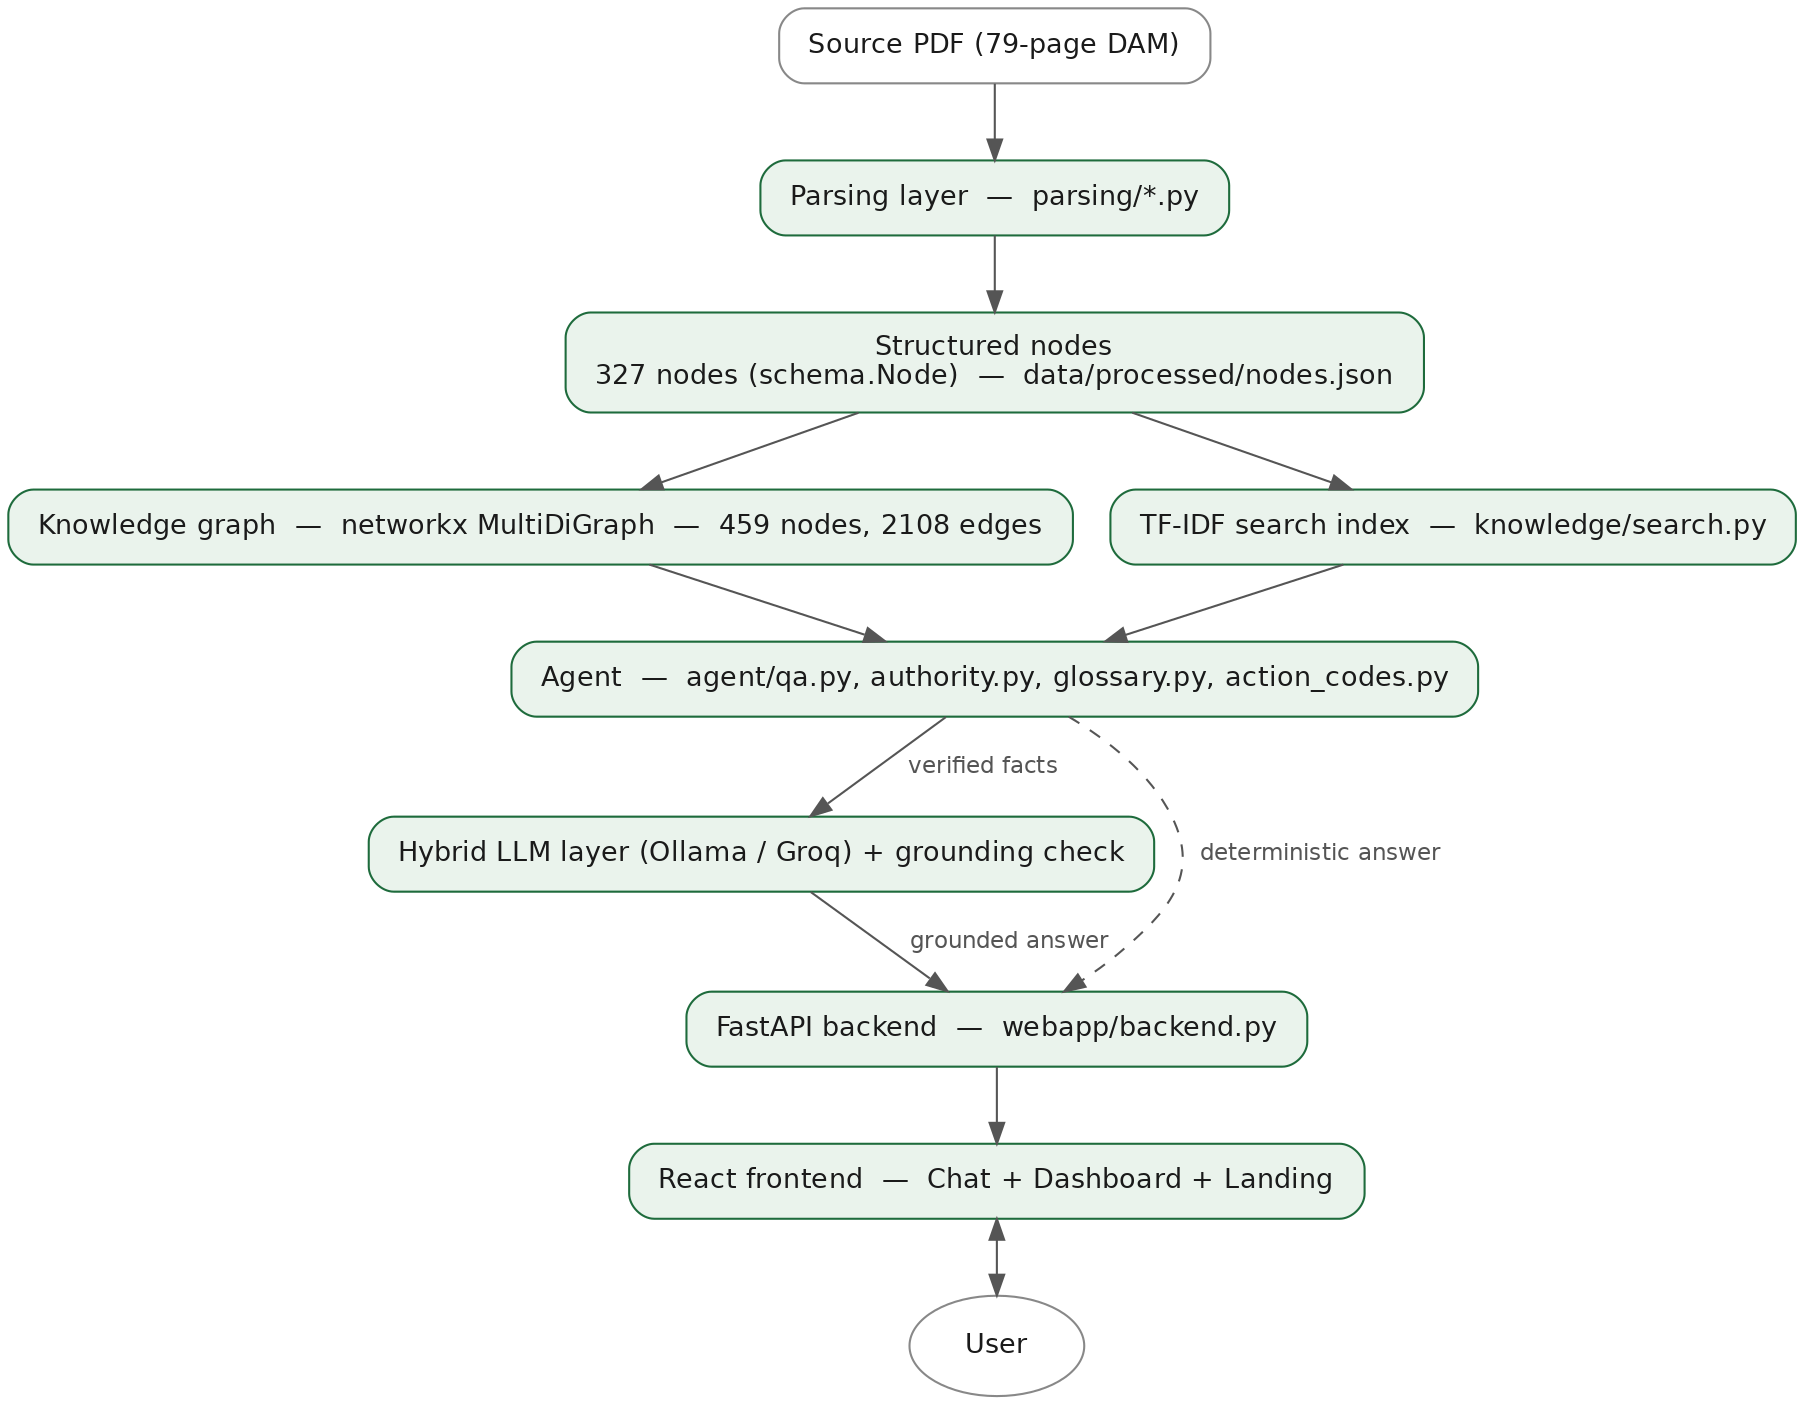
\includegraphics[width=0.82\textwidth,height=0.8\textheight,keepaspectratio]{figures/fig1_architecture.png}
\caption{Global architecture of the proposed system, from source document to user-facing answer.}
\label{fig:architecture}
\end{figure}

One consequence of this separation is worth noting early. Because extraction happens offline and its output is cached, the running application never touches the PDF. It loads a prepared node set at startup, holds it in memory, and answers from it. That decision was made for deployment reasons, and Chapter~5 explains what happened when it was not made.

\subsection{Selected Technologies}

\begin{longtable}{|p{0.26\textwidth}|p{0.62\textwidth}|}
\caption{Selected technologies and their role in the system.}\label{tab:tech}\\
\hline
\rowcolor{myblue}\textcolor{white}{\textbf{Technology}} & \textcolor{white}{\textbf{Role in the system}} \\
\hline
\endfirsthead
\hline
\rowcolor{myblue}\textcolor{white}{\textbf{Technology}} & \textcolor{white}{\textbf{Role in the system}} \\
\hline
\endhead
Python & Language for extraction, knowledge base, agent, and backend. \\ \hline
pdfplumber & Character- and word-level PDF extraction with positional coordinates, which is what makes geometric reasoning about rotated headers and superscripts possible. \\ \hline
Pydantic & Schema definition and validation for the node model, so malformed records fail at construction rather than at query time. \\ \hline
networkx & Knowledge graph construction and traversal, using a directed multigraph so that a role can hold several distinct responsibilities over the same activity. \\ \hline
scikit-learn & TF-IDF vectorisation and cosine similarity for free-text activity resolution. \\ \hline
FastAPI & REST backend, chosen for its typed request and response models and automatic API documentation. \\ \hline
React and Vite & Web client, built as a single-page application and served as static files by the backend. \\ \hline
Groq and Ollama & Language model providers for answer phrasing, cloud-hosted and local respectively, behind a common interface so either can be used or neither. \\ \hline
Web Speech API & Browser-native speech recognition for voice input, requiring no server-side audio processing. \\ \hline
python-jose and passlib & JSON Web Token issuing and password hashing for the authentication layer. \\ \hline
ReportLab & Server-side PDF generation for conversation export. \\ \hline
statsmodels & Time-series decomposition and forecasting for the analytics layer. \\ \hline
Docker & Containerisation, so the application runs identically in development and in deployment. \\ \hline
Render & Hosting platform, used on its free tier. \\ \hline
\end{longtable}

\section*{Conclusion}
\addcontentsline{toc}{section}{Conclusion}

The DAM answers an important question, and the way it is published makes that answer expensive to retrieve. Manual consultation is slow and error-prone because the document's meaning lives in its layout, and generic document assistants fail for the same reason, with the added risk that they fail fluently. The requirements set out above respond to both problems, and the architecture proposed in response separates fact retrieval from phrasing so that the flexibility of a language model can be used without inheriting its unreliability. The next chapter turns to the source document itself and examines, in detail, what makes extracting it difficult.
